\begin{example}[Advection 1D]
\label{ex:adv1D}
In $\Omega = \langle 0, 1 \rangle$ we will solve equation \eqref{eq:ex_advection}.
%\begin{equation}
%\pdiff{u}{t} + \fdiff{u}{x} = 0.
%\end{equation}
We set two the initial conditions $u(0, x)$ to obtain two different solutions:
\begin{equation}
u_{smooth} = \begin{cases}
g(x),\quad &0.1 < x < .3\\
0, \quad &\text{elsewhere}
\end{cases}
\end{equation}
where
\begin{equation}
g(\xi) = \exp\left(\frac{1}{10(\xi - 0.2)^2 - 1}+ 1\right),
\end{equation}
and
\begin{equation}
u_{step} = \begin{cases}
\dfrac{1}{2},\quad &0.1 < x < .3\\
0, \quad &\text{elsewhere}
\end{cases}.
\end{equation}
And prescribe periodic boundary condition at $x = 0 $ and $x = 1$  this 
results in the solution at time $t = 1$ to be the same as initial condition 
i.e.
\begin{equation}
u(1, x) = u(0, x).
\end{equation} 
%First we evaluate approximation of initial condition. As seen from figure 
%\ref{fig:conv_0adv1D} the approximation corresponds to theoretical orders.
We then compare these to test the convergence, see Figures 
\ref{fig:adv_conv_1D} and \ref{fig:adv_conv_1D_step}. For smooth initial condition 
limiting increases error of the solution due to artificial diffusion, higher order 
methods are capable of counteracting this effect though. For discontinuous initial 
condition limiting significantly improves behavior of the method removing oscillations 
and basically enabling use of high order methods, which suffer from them the most. The 
resulting errors are still significant as limiting introduces prominent 
smoothing. Note that for both $u_{smooth}$ a $u_{step}$ with and without limiting the 
convergence rate of the method is impacted by used 3rd order TVD Runge-Kutta 
time-stepping solver. 
\end{example}

\begin{figure}[h!]
	\centering
	\begin{subfigure}{.5\textwidth}	
		\centering	
		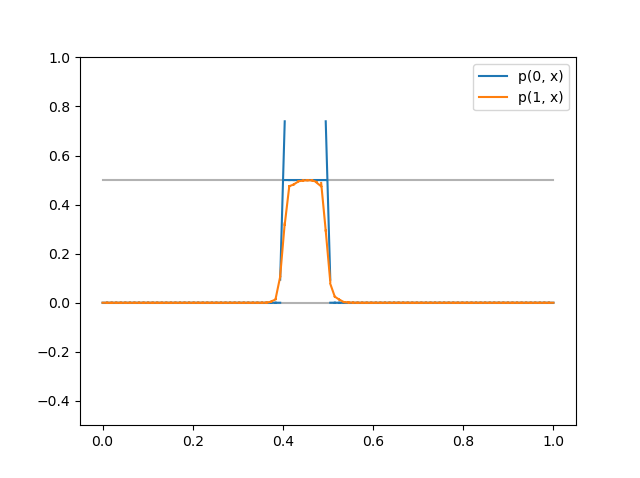
\includegraphics[width=\linewidth]{../figs/sols/adv1d_o2h100_limit}
		\caption{Limit: True}
	\end{subfigure}%
	\begin{subfigure}{.5\textwidth}
		\centering	
		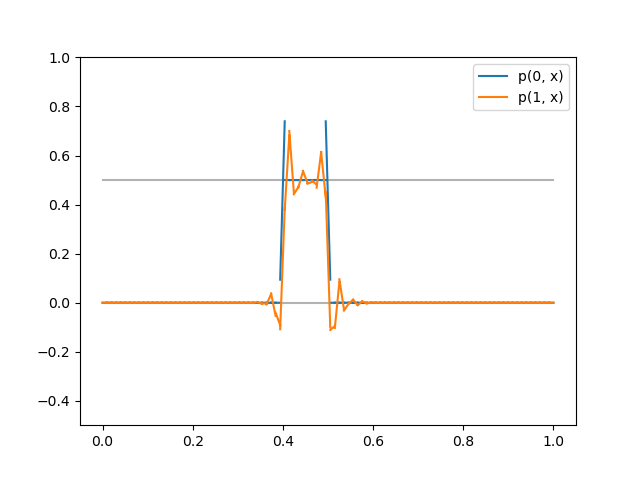
\includegraphics[width=\linewidth]{../figs/sols/adv1d_o2h100_nolimit}
		\caption{Limit: False}
	\end{subfigure}
	\caption{\Cref{ex:adv1D} Solution for $u_{step}$ for CFL coefficient $c=0.1$}
	\label{fig:sol_adv1D} 
\end{figure}

\begin{figure}[p!]
	\centering
	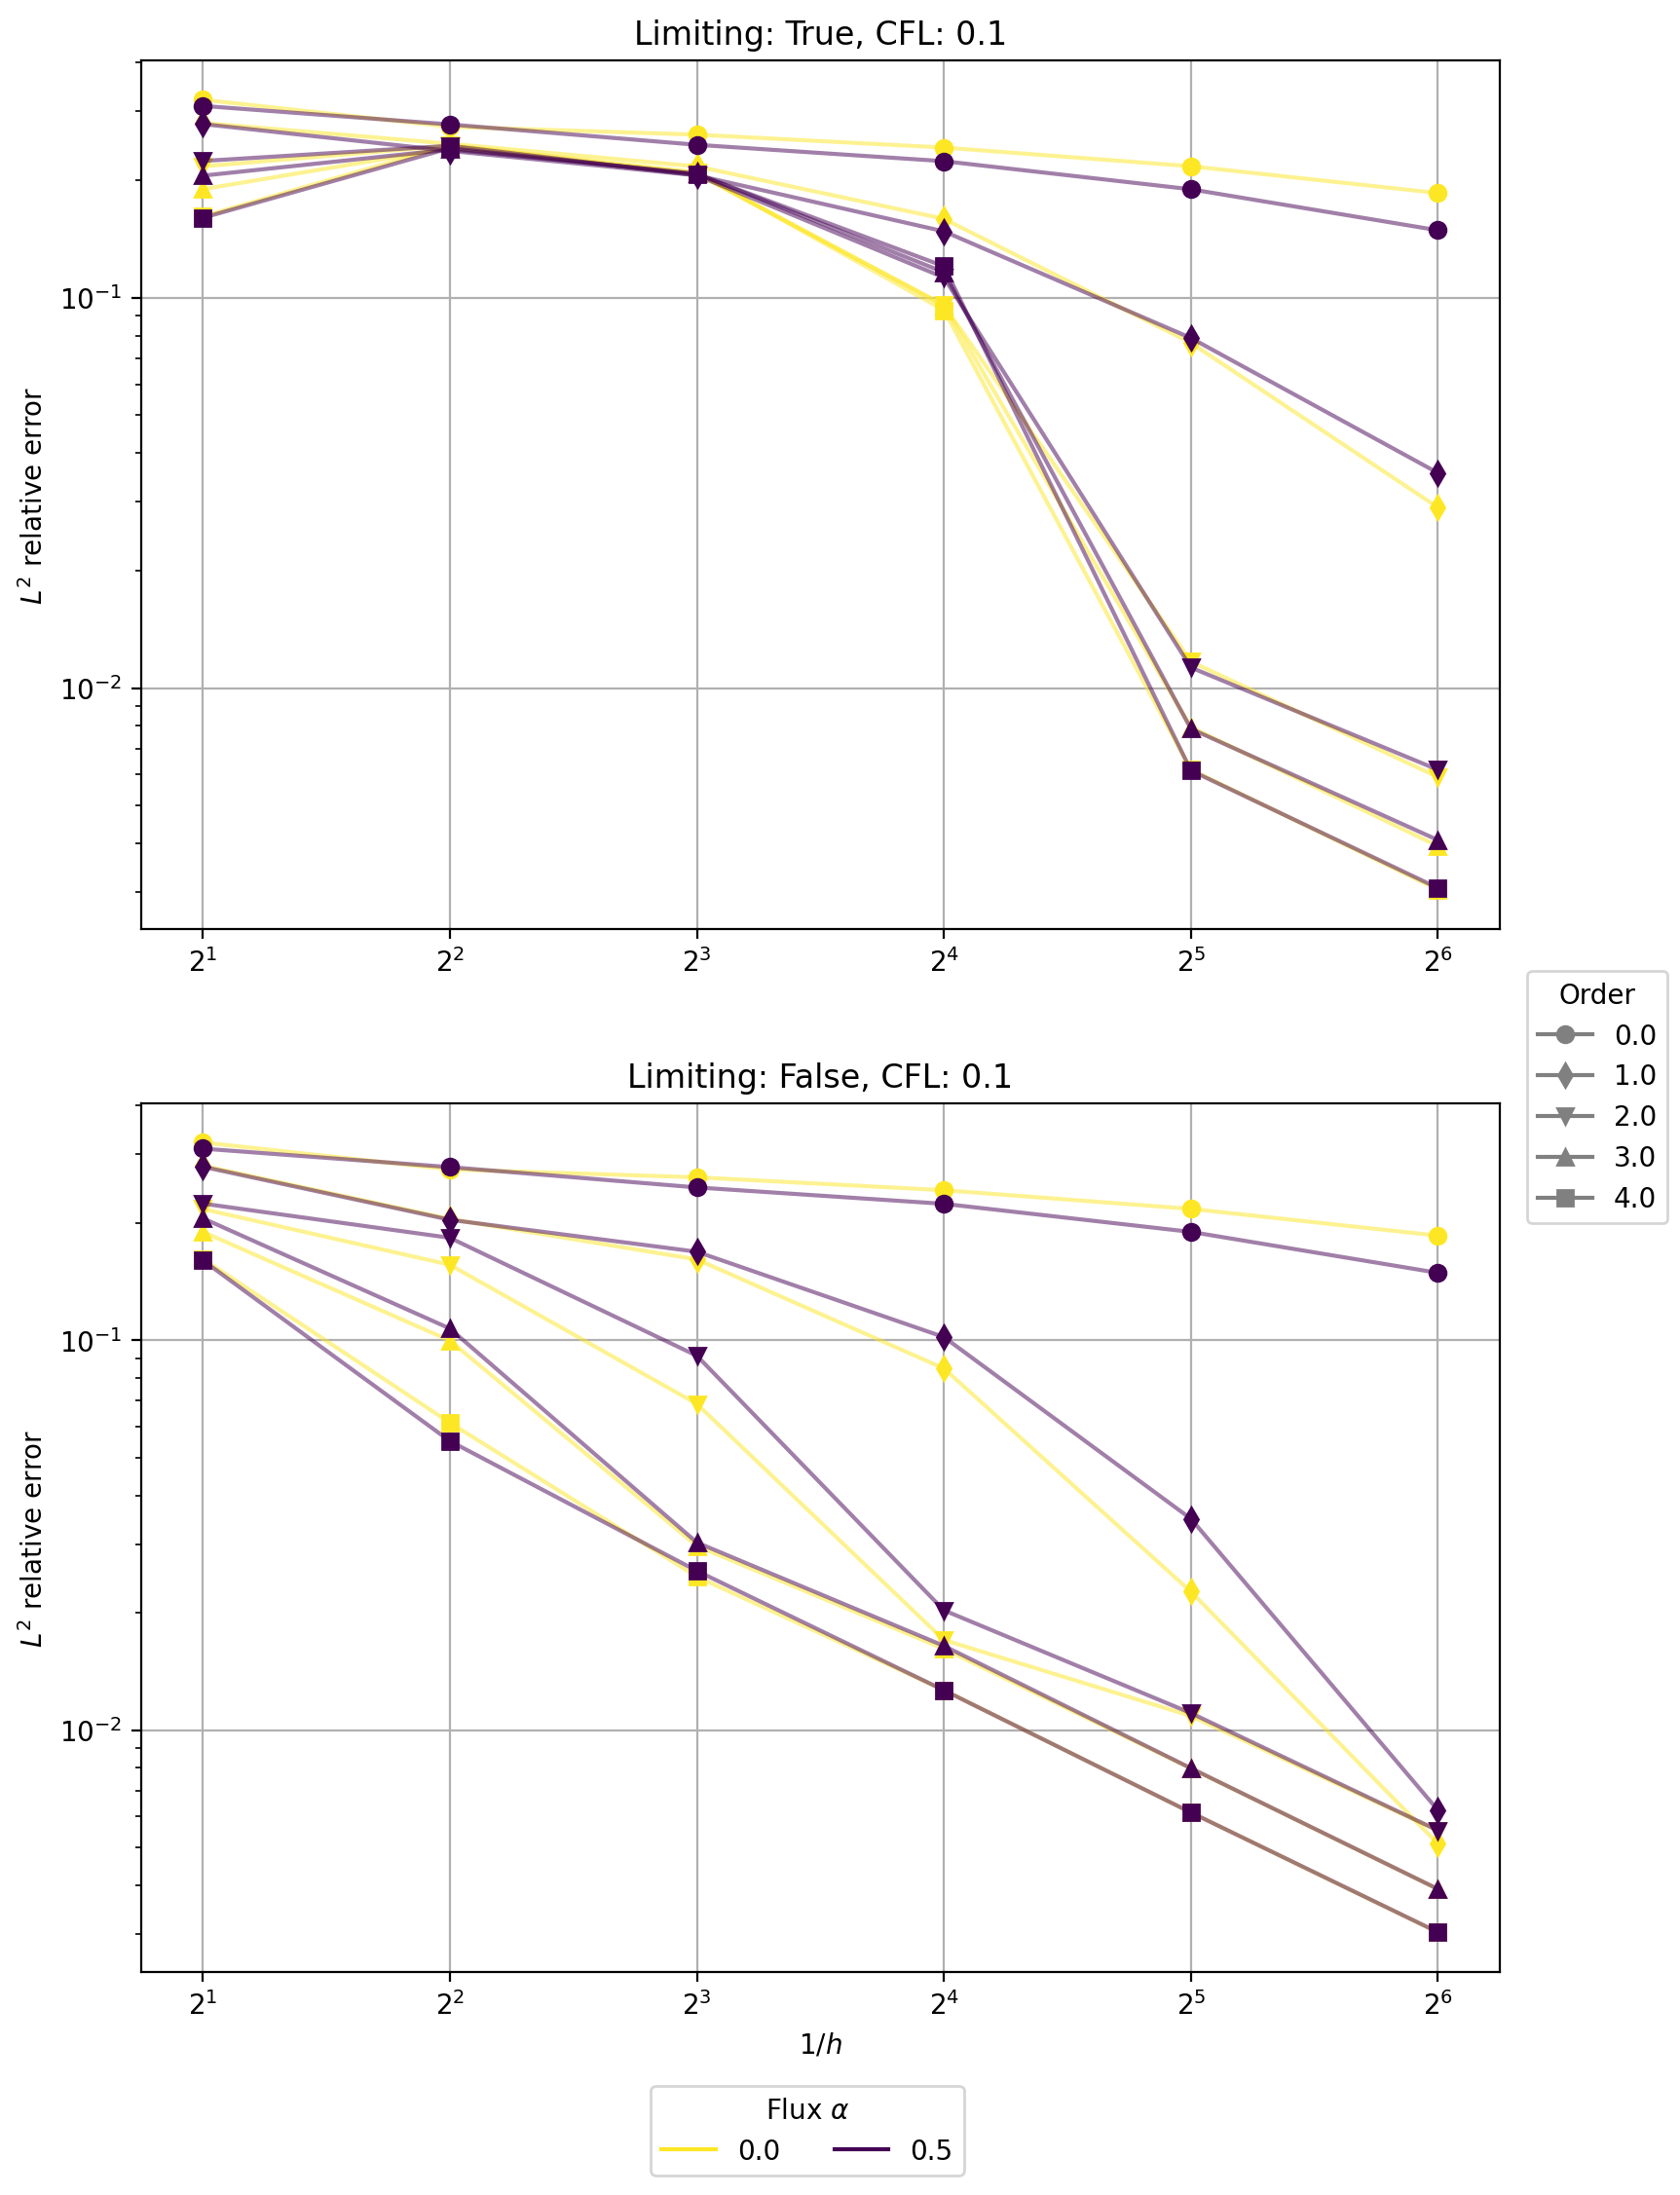
\includegraphics[width=1.1\textwidth]{../figs/parametric/advection_1D/advection_1D_smooth_reduced.png}
	\caption{\Cref{ex:adv1D} convergence plots for smooth initial condition 
		$u_{smooth}$}
	\label{fig:adv_conv_1D}
\end{figure}


\begin{figure}[p!]
	\centering
	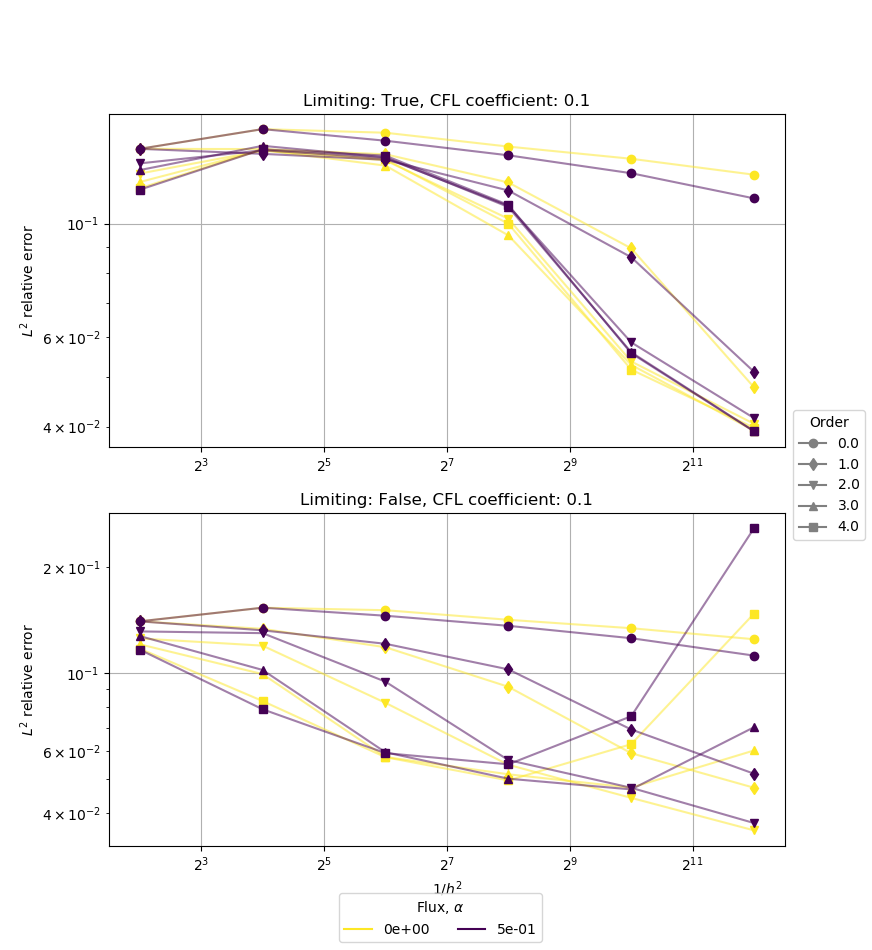
\includegraphics[width=1.1\textwidth]{../figs/parametric/advection_1D/advection_1D_step_reduced.png}
	\caption{\Cref{ex:adv1D} convergence plots for discontinuous initial 
	condition $u_{step}$}
	\label{fig:adv_conv_1D_step}
\end{figure}
